\scanpage{23}
\figure{
\begin{tikzpicture}\node[draw,circle] {$\mspage{\unsure{e|c}}$};\end{tikzpicture}}
\diagram{\begin{tikzcd}[column sep=large,row sep=huge]
X \arrow[r,bend left=24,"g_0=\varphi i"{name=t}]
  \arrow[r,bend right=24,"g_1=g"'{name=b}] \arrow[d,"i"'] & Y \arrow[d,"p"]\\
X' \arrow[ur,-,bend left=18,"\theta_0=\varphi"]
   \arrow[ur,dashed,"\theta_1=\bar\varphi"']
   \arrow[r,bend left=24,"g'_0=p\varphi"{name=u}]
   \arrow[r,bend right=24,"g'_1=g'"'{name=v}] & Y'
\arrow[from=t,to=b,"k"',shorten <=3pt,shorten >=3pt]
\arrow[from=b,to=t,shift right=8pt,shorten <=4pt,shorten >=4pt]
\arrow[from=u,to=v,"\unsure{h}"',shorten <=3pt,shorten >=3pt]
\arrow[from=v,to=u,shift left=8pt,shorten <=4pt,shorten >=4pt]
\end{tikzcd}}
We know \inserted{by assumption} there exist \inserted{simplicial} homotopies
\[
k:g_0=\varphi i\longrightarrow g_1=g\qquad\unsure{\text{and}}
\]
\[
h:g'_0=p\varphi\longrightarrow g'_1=g'.
\]
All we have to do, is to check that we can choose these homotopies \uline{compatible} with $i$ and $p$.
\margin{But in case $Y'$ is the final object, \deleted{\unsure{considering that}} \inserted{we are through!}}
\figure{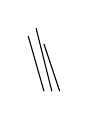
\begin{tikzpicture}\draw (0,0)--(-.2,.7);\draw (.1,0)--(-.1,.8);\draw (.2,0)--(0,.6);\end{tikzpicture}}
\deleted{\diagram{\begin{tikzcd}[column sep=small]
(X\amalg X) \arrow[d,"\mathrm{cofib?}"] & \amalg & (X'\amalg X') \arrow[d,"\mathrm{cofib?}"',"\unsure{=}"]\\
X\otimes J & \amalg \arrow[d] & X'\otimes J \arrow[r] & (Y\otimes J)\amalg\unsure{\bar\theta}\\
Y & \amalg & Y'
\end{tikzcd}}}
diagram
\diagram{\begin{tikzcd}
X\otimes J \arrow[r,"k"] \arrow[d,"i\otimes J"'] \arrow[dr,bend left=9] \arrow[dr,bend right=9] & Y \arrow[d,"p"]\\
X'\otimes J \arrow[r,"h"'] & Y'
\end{tikzcd}}
\deleted{which a priori is \uline{not} commutative but only commutative \deleted{\unsure{for}} on $X\amalg X\longrightarrow X\otimes J$}
\deleted{\diagram{\begin{tikzcd}
X\otimes J \arrow[r,"k"] \arrow[d,"i\otimes J"'] & Y \arrow[d,"p"]\\
X'\otimes J \arrow[r,"h"'] & Y'
\end{tikzcd}}}
\deleted{\diagram{\begin{tikzcd}[row sep=large]
X\amalg X \arrow[d] \arrow[dr,bend left=18,"u=(g_0,g_1)"] & \\
X\otimes J \arrow[r,dashed,-,"h'!"] \arrow[d,"i\otimes J"'] & Y \arrow[d,"p"]\\
X'\otimes J \arrow[r,"h"'] & Y'
\end{tikzcd}}}
\deleted{This diagram is commutative and we look for $h'$ which keeps it commutative.}
\deleted{We invert the problem, \deleted{\unsure{forgetting}} \inserted{\unsure{shortcircuiting}} $X'\otimes J$ by the arrow $h\circ(i\otimes J)=v$.}
\deleted{We know there is a \deleted{\unsure{and we want a}} $k$ s.th. $kj=u$, but \unsure{unfortunately} $ph\ne v$; only $pk\overset{s}{\sim}v$}
\deleted{(But in case $Y'$ is final object, we are already through!)}
\deleted{\diagram{\begin{tikzcd}
X\amalg X \arrow[r,"u=(g_0,g_1)"] \arrow[d,"j", "\text{\uuline{non} trivial cofibration}"'] & Y \arrow[d,"p\ \text{fibration}"]\\
X\otimes J \arrow[r,"v"'] \arrow[ur,dashed,"h'?"] & Y'
\end{tikzcd}}}
\margin{\deleted{\unsure{\times 0}}}
\figure{\begin{tikzpicture}[scale=.6]
\draw (0,12)--(2,13);\draw (0,10)--(4,13);\draw (0,7)--(1,8);
\draw (1,8)--(6,11);\draw (3,13)..controls(4,12.7)and(5,12.5)..(5.5,12);
\draw (0,6)--(8,-1);\draw (2,-1)--(10,8);
\end{tikzpicture}}
\mspage{22}
